\subsection{Desarrollo teórico}
\label{subsec:desarrollo}
En la sección de desarrollo teórico trataré de proporcionar un procedimiento mediante el cual los alumnos que realicen la práctica sean capaces de optimizar la velocidad y fuerza del proyectil a partir de los parámetros eléctricos y geométricos que definen el sistema. Estos parámetros de entrada serán:
\begin{itemize}
    \item \textbf{Parámetros geométricos}:
    \begin{enumerate}[label=\alph*., leftmargin=*, itemindent=1em]
        \item \(r_{cext}\) y \(r_{cint} \) : radios exterior e interior de la bobina, respectivamente.
        \item \(l_c\): altura de la bobina.
        \item \(r_{fe}\): radio del vástago.
        \item \(l_{fe}\): longitud del vástago.
    \end{enumerate}
    \item \textbf{Parámetros eléctricos}:
    \begin{enumerate}[label=\alph*., leftmargin=*, itemindent=1em]
        \item \(N\): número de espiras.
        \item \(I_{cc}\): corriente de alimentación del solenoide.
        \item \(\mu_{fe}\): permeabilidad relativa del vástago ferromagnético.
    \end{enumerate}
\end{itemize}

El objetivo de este desarrollo es crear un programa en MATLAB al que se le proporcionen estos datos, y que calcule automáticamente la fuerza que experimentará el proyectil. Como se muestra en la figura \ref{fig:electromagnet} el valor de
\(B\) varía a lo largo del solenoide. Por lo tanto, además de los parámetros dados (que son constantes), será necesario parametrizar también la posición del vástago en cada momento y calcular la fuerza que experimenta en cada una de esas posiciones. Con todo esto, he desarrollado el siguiente esquema que muestra las variables del sistema:

\begin{figure}[H]
    \centering
    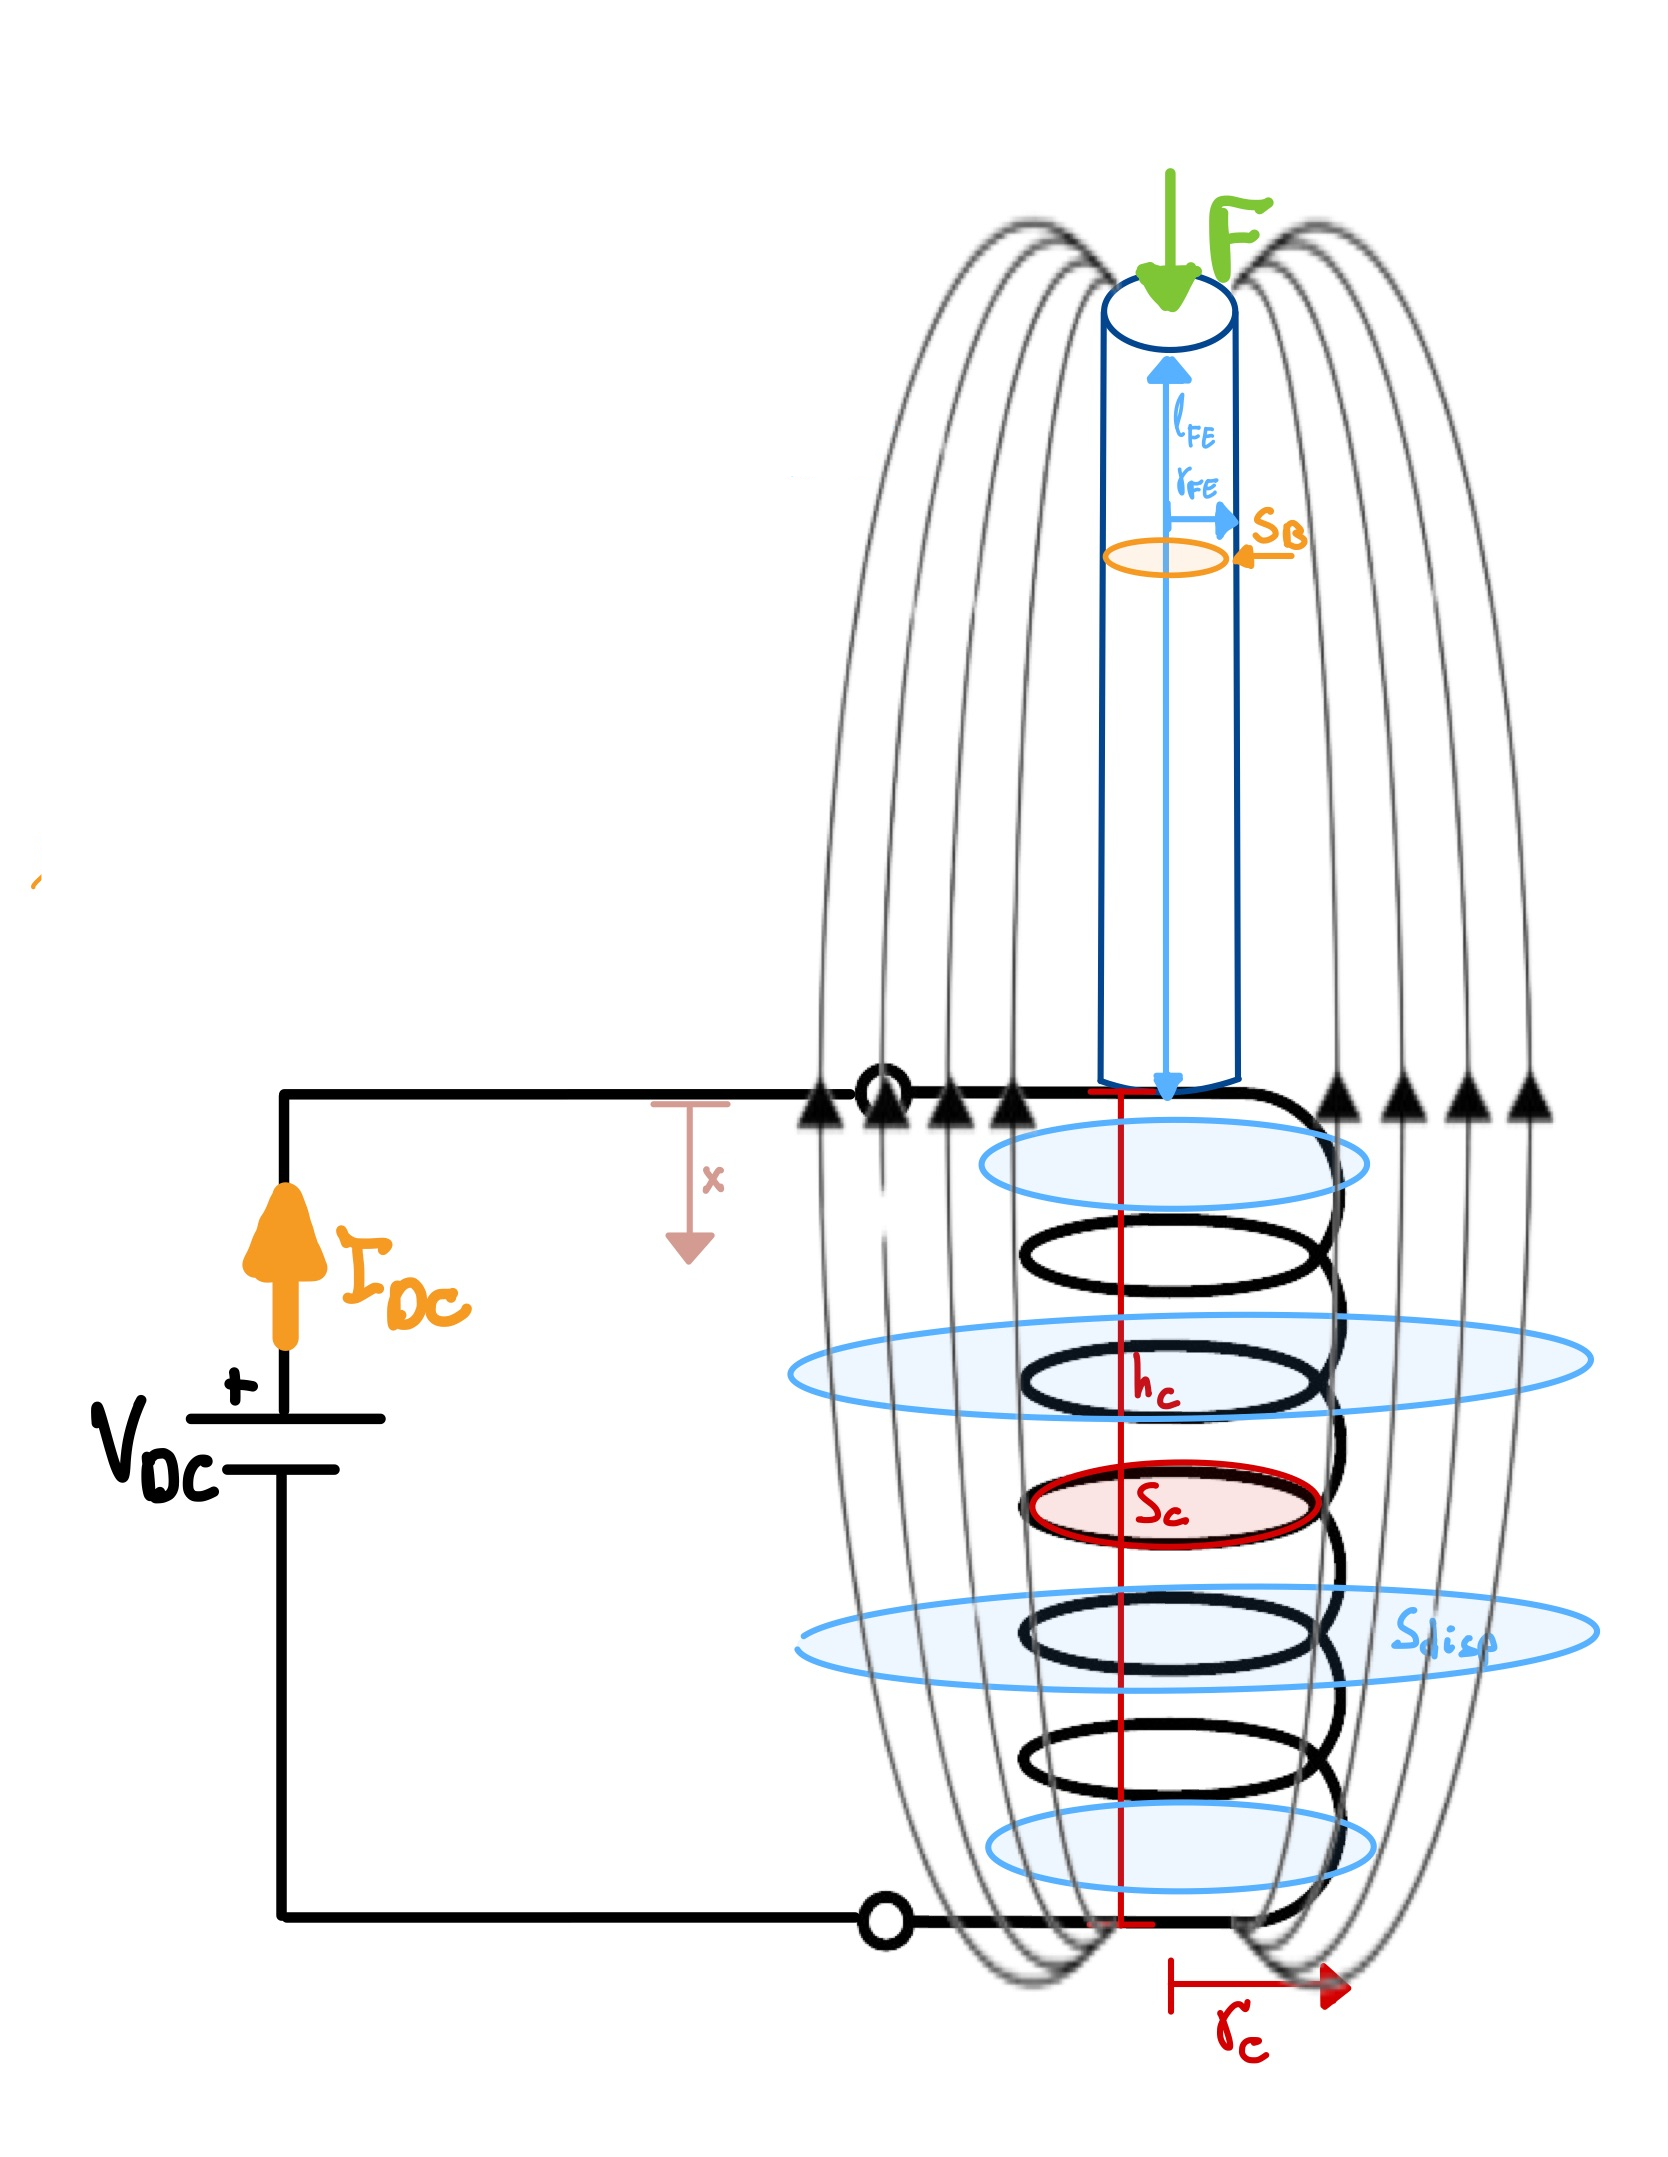
\includegraphics[width=7cm]{FigurasMemoria/esquemaDesTeor.png}
    \caption{Esquema geométrico del sistema. Elaboración propia.}
    \label{fig:esquemaDesTeor} %Para referenciar -> \ref{fig:figNum}
\end{figure}

Antes de empezar a escribir el código, tenemos que realizar un desarrollo analítico partiendo de las fórmulas del marco teórico. Mi idea para conseguir un valor de la fuerza que se pueda calcular y programar fácilmente es conseguir un circuito magnético equivalente que exprese las principales reluctancias del sistema. La reluctancia es un concepto análogo a la resistencia eléctrica, solo que para el flujo magnético \citep{hughes2005electrical}. Todos los materiales tienen reluctancia magnética y su expresión es:

\begin{center}
    \[\mathcal{R} = \frac{l_{caract}}{\mu_0*\mu_r*S_{efect}}\]
\end{center}

Como se puede observar, el valor de la reluctancia depende de la geometría del cuerpo del que se esté calculando, por lo que a a ser el parámetro que nos relaciones los valores métricos del sistema con los eléctricos.

Además de este valor, también podemos definir la \textit{Fuerza Electromotriz} o \textit{FFM}, un parámetro análogo a la tensión en un circuito eléctrico, que en un solenoide es el resultado de multiplicar el número de espiras por su corriente de alimentación:

\begin{center}
    \[\mathcal{F}=NI\]
\end{center}

Combinando estas dos ecuaciones obtenemos la expresión del flujo en un solenoide, que consecuentemente es el análogo a la corriente en un circuito eléctrico:

\begin{center}
    \[\phi=\frac{\mathcal{F}}{\mathcal{R}}=\frac{NI}{\mathcal{R}}\]
\end{center}

Y para terminar, la inducción magnética \(B\) se corresponde con el flujo magnético que fluye a través de un área del espacio, por lo que podemos escribir:

\begin{center}
    \[B=\phi S\to B=\frac{NIS}{\mathcal{R}}\]
\end{center}

Al tener una expresión de la inducción en función de la reluctancia, ya hemos conseguido una fórmula que nos proporciona la cantidad de campo generado a partir de las diferentes variables de entrada. Solo necesitamos otra expresión que nos devuelva la fuerza dinámica a partir de la inducción. Según Nicolás Jerez \citep{jerez2016resueltos} la fuerza de atracción para un flujo constante y un circuito magnético lineal es:
\begin{center}
\[F=\frac{1}{2}\frac{B^2*S}{\mu_0}\]
\end{center}

Por lo que la relación queda definida. Tenemos la capacidad de obtener la fuerza a la que va a ser disparado el proyectil a partir de la geometría y valores de alimentación del sistema.